% --------------------------------------------------------------------------------------------------------------
% --------------------------------------------------------------------------------------------------------------
% --------------------[ "A (very) short introduction to R" - Paul Torfs & Claudia Brauer ]----------------------
% --------------------------------------------------------------------------------------------------------------
% --------------------------------------------------------------------------------------------------------------
% --- Current file is a modified version of the original TeX file of the tutorial, which was written by Paul ---
% --- Torfs & Claudia Brauer. It's the basic file for the greek translation.                                 ---
% --------------------------------------------------------------------------------------------------------------
% --------------------------------------------------------------------------------------------------------------


% --------------------------------------------------------------------------------------------------------------
% Document specifications. -------------------------------------------------------------------------------------
\documentclass[a4paper,10pt,twocolumn]{article}
\usepackage[top=2.4cm, bottom=2.4cm, left=2cm, right=2cm]{geometry}
% --------------------------------------------------------------------------------------------------------------

% --------------------------------------------------------------------------------------------------------------
% General packages. --------------------------------------------------------------------------------------------
\usepackage{amssymb}
\usepackage{wasysym}
\usepackage{multicol}
\usepackage{multirow}
\usepackage{hyperref}
\usepackage{url}
\usepackage{graphicx}
\usepackage{caption}
\captionsetup[figure]{labelfont=bf}
% --------------------------------------------------------------------------------------------------------------

% --------------------------------------------------------------------------------------------------------------
% Packages for boxes with code. --------------------------------------------------------------------------------
\usepackage{fancybox}
\usepackage{fvrb-ex}
% --------------------------------------------------------------------------------------------------------------

% --------------------------------------------------------------------------------------------------------------
% Additional packages for greek language. ----------------------------------------------------------------------
\usepackage{fontspec}
\usepackage{xunicode}
\usepackage{xltxtra}
\usepackage{xgreek}
\setmainfont[Mapping=TeX-text]{Arial}
% --------------------------------------------------------------------------------------------------------------

% --------------------------------------------------------------------------------------------------------------
% The ToDo environment. ----------------------------------------------------------------------------------------
\usepackage[usenames,dvipsnames]{color}
 \newenvironment{ToDo} {
  \begin{flushright}
    \hfill
    \begin{minipage}{0.9\columnwidth}
    \textsf{\textbf{ToDo}} \\
      \vspace{-0.7cm}\\
      {\color{Gray}\rule[-0.05cm]{\columnwidth}{1.5pt}}} {
      {\color{Gray}\rule[0.3cm]{\columnwidth}{1.5pt}}
    \end{minipage}
    \vspace{0.3cm}
  \end{flushright}
  }
% --------------------------------------------------------------------------------------------------------------

% --------------------------------------------------------------------------------------------------------------
% Footnote modifications. --------------------------------------------------------------------------------------
\makeatletter
\newcommand{\noun}[1]{\textsc{#1}}
%% Special footnote code from the package 'stblftnt.sty'
%% Author: Robin Fairbairns -- Last revised Dec 13 1996
\let\SF@@footnote\footnote
\def\footnote{\ifx\protect\@typeset@protect
 \expandafter\SF@@footnote
 \else
 \expandafter\SF@gobble@opt
 \fi
}
\expandafter\def\csname SF@gobble@opt \endcsname{\@ifnextchar[%]
 \SF@gobble@twobracket
 \@gobble
}
\edef\SF@gobble@opt{\noexpand\protect
 \expandafter\noexpand\csname SF@gobble@opt \endcsname}
\def\SF@gobble@twobracket[#1]#2{}
\makeatother
% --------------------------------------------------------------------------------------------------------------

% --------------------------------------------------------------------------------------------------------------
% Improve float handling. --------------------------------------------------------------------------------------
\renewcommand{\topfraction}{0.9}	
 \renewcommand{\bottomfraction}{0.8}	
 \setcounter{topnumber}{2}
 \setcounter{bottomnumber}{2}
 \setcounter{totalnumber}{4} 
 \setcounter{dbltopnumber}{2} 
 \renewcommand{\dbltopfraction}{0.9}	
 \renewcommand{\textfraction}{0.07}	
 \renewcommand{\floatpagefraction}{0.7}	
	% floatpagefraction MUST be less than topfraction !!
 \renewcommand{\dblfloatpagefraction}{0.7}
% --------------------------------------------------------------------------------------------------------------


% --------------------------------------------------------------------------------------------------------------
% Notes on formatting. -----------------------------------------------------------------------------------------
% - \texttt{...} is used to emphasize commands or clicking buttons in verbatim.
% - \verb!...! is only used instead of \texttt{...} when there are brackets or other things
%   \texttt can't handle.
% - \emph{...} is used to emphasize new terms
% --------------------------------------------------------------------------------------------------------------


% --------------------------------------------------------------------------------------------------------------
% Title of the document. ---------------------------------------------------------------------------------------
\title{\vspace{-13mm} \textbf{Μια (πολύ) σύντομη εισαγωγή στην R}}
\author{Paul Torfs \& Claudia Brauer\\
\small{Ομάδα Υδρολογίας \& Ποσοτικής Διαχείρισης Υδάτων}\\
\small{Πανεπιστήμιο Wageningen, Ολλανδία}}
\date{\small{4 Νοεμβρίου 2014}}
% --------------------------------------------------------------------------------------------------------------


\begin{document}
\maketitle


% --------------------------------------------------------------------------------------------------------------
% [#01] Introduction
% --------------------------------------------------------------------------------------------------------------
\section{Εισαγωγή}

Η R είναι μια ισχυρή γλώσσα και ένα ισχυρό περιβάλλον ανάπτυξης για στατιστικούς
υπολογισμούς και γραφικά. Ως έργο αποτελεί κοινό κτήμα (ή αλλιώς, είναι GNU project),
και είναι παρόμοια με την εμπορική γλώσσα και περιβάλλον S, που είχε αναπτυχθεί στα Bell 
Laboratories (πρώην AT\&T, πλέον Lucent Technologies) από τον John Chambers και τους συνεργάτες
του. Η R μπορεί να θεωρηθεί πως είναι μια διαφορετική υλοποίηση της S, και χρησιμοποιείται ευρέως
ως εκπαιδευτική γλώσσα και ως ερευνητικό εργαλείο.

Τα κύρια πλεονεκτήματα της R είναι το γεγονός ότι η R είναι ελεύθερο λογισμικό και ότι υπάρχει
πολύ βοήθεια διαθέσιμη στο διαδίκτυο. Είναι αρκετά παρόμοια με άλλα προγραμματιστικά πακέτα όπως 
η MATLAB (που δεν είναι ελεύθερο λογισμικό), αλλά πιο φιλική προς τον χρήστη από γλώσσες
προγραμματισμού όπως η C++ και η Fortran. Μπορείτε να χρησιμοποιήσετε την R όπως είναι, αλλά για
εκπαιδευτικούς λόγους εμείς προτιμούμε τη χρήση της R σε συνδυασμό με την διεπαφή του RStudio
(που είναι κι αυτό ελεύθερο λογισμικό), το οποίο έχει μια οργανωμένη διάταξη και διάφορες πρόσθετες
επιλογές.

Το παρόν έγγραφο περιλαμβάνει επεξηγήσεις, παραδείγματα και ασκήσεις, τα οποία (ελπίζουμε ότι)
μπορούν να γίνουν κατανοητά από ανθρώπους που δεν έχουν κάποια προγραμματιστική εμπειρία. Το διάβασμα
όλου του κειμένου και των ασκήσεων απαιτεί περίπου 1 με 2 ώρες. Παραδείγματα από εντολές, που 
χρησιμοποιούνται συχνά, και από μηνύματα λάθους παρατίθενται στις τελευταίες δύο σελίδες αυτού
του εγγράφου και μπορούν να χρησιμοποιηθούν ως αναφορά κατά τον προγραμματισμό.
% --------------------------------------------------------------------------------------------------------------


% --------------------------------------------------------------------------------------------------------------
% [#02] Getting started
% --------------------------------------------------------------------------------------------------------------
\section{Ξεκινώντας}

% ----- [01] Install R -----------------------------------------------------------------------------------------
\subsection{Εγκατάσταση της R}

Για να εγκαταστήσετε την R στον υπολογιστή σας (δωρεάν και με νόμιμο τρόπο!), πηγαίνετε στην
αρχική σελίδα του ιστοτόπου της R\footnote{Στον ιστότοπο της R μπορείτε επίσης να βρείτε και το παρόν έγγραφο:
\url{http://cran.r-project.org/doc/contrib/Torfs+Brauer-Short-R-Intro.pdf}}:
\begin{quote}
  \url{http://www.r-project.org/}
\end{quote}
και εκτελέστε τα ακόλουθα (υποθέτοντας ότι δουλεύετε σε έναν υπολογιστή με Windows):\\
\noindent $\bullet$ κάντε κλικ στο \texttt{download CRAN} στην αριστερή στήλη\\
\noindent $\bullet$ επιλέξτε έναν ιστότοπο  απ' όπου θα γίνει η λήψη\\
\noindent $\bullet$ επιλέξτε \texttt{Windows} ως λειτουργικό σύστημα\\
\noindent $\bullet$ κάντε κλικ στο \texttt{base}\\
\noindent $\bullet$ επιλέξτε \texttt{Download R 3.0.3 for Windows} \footnote{Τη στιγμή της
συγγραφής του κειμένου αυτού η τελευταία έκδοση ήταν η 3.0.3. Επιλέξτε την πιο πρόσφατη.} και
αφήστε τις προεπιλεγμένες απαντήσεις σε όλες τις ερωτήσεις\\

Είναι επίσης δυνατόν να εκτελέσετε την R και το RStudio μέσω ενός USB αντί να τα εγκαταστήσετε. Αυτό
θα μπορούσε να φανεί χρήσιμο όταν δεν έχετε δικαιώματα διαχειριστή στον υπολογιστή σας. Δείτε και 
την ξεχωριστή σημείωσή μας ``How to use portable versions of R and RStudio" για βοήθεια στο 
συγκεκριμένο θέμα.

% ----- [02] Install RStudio -----------------------------------------------------------------------------------
\subsection{Εγκατάσταση του RStudio}

Μετά την ολοκλήρωση της εγκατάστασης, θα πρέπει να βλέπετε ένα εικονίδιο ``R" στην επιφάνεια
εργασίας σας. Κάνοντας κλικ σε αυτό θα εκκινήσετε την τυπική διεπαφή. Εμείς θα σας συνιστούσαμε,
ωστόσο, να χρησιμοποιήσετε την διεπαφή του RStudio. \footnote{Υπάρχουν πολλές άλλες διεπαφές
(ελεύθερου λογισμικού), όπως το Tinn-R.} Για να εγκαταστήσετε το RStudio, πηγαίνετε στον ιστότοπο: 
\begin{quote}
  \url{http://www.rstudio.org/}
\end{quote}
και εκτελέστε τα ακόλουθα βήματα (υποθέτοντας ότι δουλεύετε σε έναν υπολογιστή με Windows):\\
\noindent $\bullet$ κάντε κλικ στο \texttt{Download RStudio}\\
\noindent $\bullet$ κάντε κλικ στο \texttt{Download RStudio Desktop}\\
\noindent $\bullet$ κάντε κλικ στο \texttt{Recommended For Your System}\\
\noindent $\bullet$ κατεβάστε το εκτελέσιμο \texttt{.exe} αρχείο και τρέξτε το 
(αφήστε τις προεπιλεγμένες απαντήσεις για όλες τις ερωτήσεις)

% ----- [03] RStudio layout ------------------------------------------------------------------------------------
\subsection{Η διάταξη του RStudio}

\begin{figure*}[htb]
  \centering
  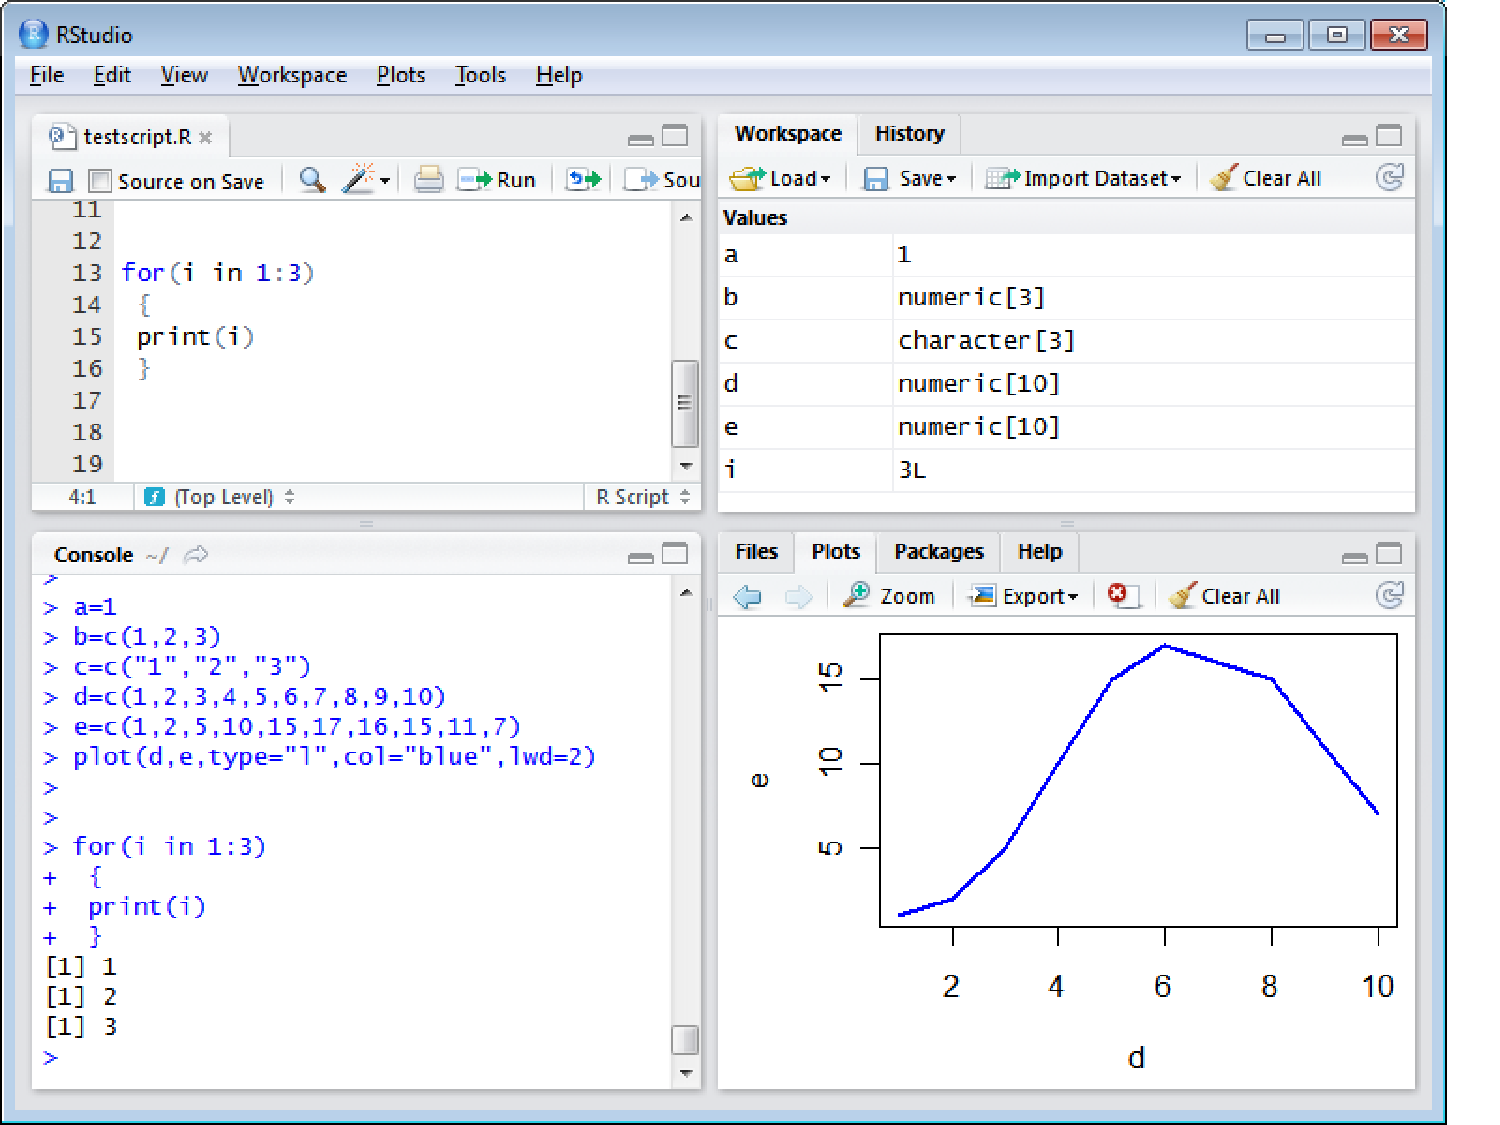
\includegraphics[width=13cm, clip=true, trim=0cm 0cm 9mm 0cm]{img/rstudio_screenshot.pdf}
  \caption{Τα παράθυρα του επεξεργαστή κειμένου (editor), του χώρου εργασίας (workspace), 
  της κονσόλας (console) και των γραφικών παραστάσεων (plots) στο RStudio.}
  \label{fig:screenshot}
\end{figure*}

Η διεπαφή του RStudio αποτελείται από διάφορα παράθυρα (βλέπε το Σχήμα~\ref{fig:screenshot}).
\begin{itemize}
\item Κάτω αριστερά: \textbf{παράθυρο κονσόλας} (καλείται επίσης και \textbf{παράθυρο εντολών}).
Εδώ μπορείτε να εισάγετε απλές εντολές μετά το σύμβολο υποβολής ``$>$'' και η R στη συνέχεια θα εκτελέσει
την εντολή σας. Αυτό είναι το πιο σημαντικό παράθυρο, επειδή στην πραγματικότητα εκεί τρέχει η R.
\item Πάνω αριστερά: \textbf{παράθυρο επεξεργαστή κειμένου} (καλείται επίσης και
\textbf{παράθυρο σεναρίων}). Εδώ μπορούν να υποστούν επεξεργασία και να σωθούν σύνολα από εντολές (σενάρια).
Όταν δεν υπάρχει αυτό το παράθυρο, μπορείτε να το ανοίξετε μέσω της διαδρομής \texttt{File} $\rightarrow$
\texttt{New} $\rightarrow$ \texttt{R script}. Η απλή πληκτρολόγηση μιας εντολής στο παράθυρο του επεξεργαστή
δεν είναι αρκετή, πρέπει επίσης να πάει και στο παράθυρο εντολών πριν η R μπορέσει να εκτελέσει την εντολή αυτή.
Εάν θέλετε να τρέξετε μία γραμμή από το παράθυρο σεναρίων (ή και ολόκληρο το σενάριο), μπορείτε να κάνετε κλικ
στο \texttt{Run} ή να πατήσετε τα πλήκτρα \texttt{CTRL+ENTER}, ώστε να τη στείλετε στο παράθυρο εντολών. 
\item Πάνω δεξιά: \textbf{χώρος εργασίας / ιστορικό}. Στο παράθυρο του χώρου εργασίας
μπορείτε να δείτε ποια δεδομένα και ποιες τιμές έχει η R στη μνήμη της. Μπορείτε να δείτε και να επεξεργαστείτε
τις τιμές κάνοντας κλικ πάνω τους. Το παράθυρο του ιστορικού δείχνει το τι έχει πληκτρολογηθεί παλιότερα. 
\item Κάτω δεξιά: \textbf{αρχεία / γραφικές παραστάσεις / πακέτα / βοήθεια}. Από εδώ μπορείτε να ανοίξετε
αρχεία, να δείτε γραφικές παραστάσεις (και προηγούμενες γραφικές παραστάσεις, επίσης), να εγκαταστήσετε
και να φορτώσετε πακέτα ή να χρησιμοποιήσετε τη λειτουργία της βοήθειας.
\end{itemize}

Μπορείτε να αλλάξετε το μέγεθος των παραθύρων σέρνοντας τα γκρίζα διαχωριστικά μεταξύ των παραθύρων.

% ----- [04] Working directory ---------------------------------------------------------------------------------
\subsection{Κατάλογος εργασίας}

Ο \emph{κατάλογος εργασίας} σας (working directory) είναι ο φάκελος του υπολογιστή σας μέσα στον οποίο
εργάζεστε. Όταν ζητήσετε από την R να ανοίξει ένα συγκεκριμένο αρχείο, αυτή θα κοιτάξει πρώτα στον κατάλογο
εργασίας γι' αυτό το αρχείο, και όταν πείτε στην R να αποθηκεύσει ένα αρχείο δεδομένων ή ένα γράφημα, αυτή
θα το αποθηκεύσει στον κατάλογο εργασίας.

Πριν ξεκινήσετε να εργάζεστε, παρακαλούμε θέστε τον κατάλογο εργασίας σας εκεί που έχετε ή εκεί που πρέπει
να αποθηκεύονται όλα τα δεδομένα σας και τα αρχεία σεναρίων.

Εισάγετε στο παράθυρο εντολών το εξής: \verb!setwd("directoryname")!. Για παράδειγμα:

\begin{Verbatim}[frame=single,gobble=0]
> setwd("M:/Hydrology/R/")
\end{Verbatim}

Σιγουρευτείτε ότι οι μπάρες είναι πλάγιες μπάρες (/) και ότι δεν έχετε ξεχάσει τις αποστρόφους (για την ανάγκη
των αποστρόφων, δείτε στην ενότητα~\ref{sec:characters}). Η R διακρίνει τα πεζά από τα κεφαλαία γράμματα, οπότε
βεβαιωθείτε ότι γράφετε με κεφαλαία εκεί που απαιτείται.

Μέσα στο RStudio μπορείτε επίσης να πάτε στο \texttt{Tools} $\rightarrow$ \texttt{Set working directory}.

% ----- [05] Libraries -----------------------------------------------------------------------------------------
\subsection{Βιβλιοθήκες} 

Η R μπορεί να κάνει πολλές στατιστικές αναλύσεις και αναλύσεις δεδομένων. Αυτές είναι οργανωμένες στα 
λεγόμενα \emph{πακέτα} ή \emph{βιβλιοθήκες}. Με την τυπική εγκατάσταση, εγκαθίστανται και τα περισσότερα
συνήθη πακέτα. 

Για να δείτε μια λίστα με όλα τα εγκατεστημένα πακέτα, πηγαίνετε στο παράθυρο πακέτων ή πληκτρολογήστε 
\verb!library()! στο παράθυρο κονσόλας. Εάν το τετραγωνάκι μπροστά από το όνομα του πακέτου είναι σημειωμένο,
το πακέτο φορτώνεται (ενεργοποιείται) και τότε μπορεί να χρησιμοποιηθεί. 

Υπάρχουν πολλά επιπλέον διαθέσιμα πακέτα στον ιστότοπο της R. Εάν θέλετε να εγκαταστήσετε και να χρησιμοποιήσετε
ένα πακέτο (για παράδειγμα, το πακέτο που λέγεται ``geometry"), τότε πρέπει να :\\
\noindent $\bullet$ Εγκαταστήσετε το πακέτο:  κάντε κλικ στο \texttt{install packages} στο παράθυρο πακέτων
και πληκτρολογήστε \texttt{geometry} ή εισάγετε την εντολή \verb!install.packages("geometry")! στο παράθυρο
εντολών.\\
\noindent $\bullet$ Φορτώστε το πακέτο: σημειώστε το κουτάκι μπροστά από το \texttt{geometry} ή εισάγετε
την εντολή \verb!library("geometry")! στο παράθυρο εντολών.
% --------------------------------------------------------------------------------------------------------------


% --------------------------------------------------------------------------------------------------------------
% [#03] Some first examples of R commands
% --------------------------------------------------------------------------------------------------------------
\section{Μερικά πρώτα παραδείγματα εντολών της R}

% ----- [01] Calculator ----------------------------------------------------------------------------------------
\subsection{Αριθμομηχανή}

Η R μπορεί να χρησιμοποιηθεί ως αριθμομηχανή. Μπορείτε απλά να εισάγετε την εξίσωση που θέλετε στο
παράθυρο εντολών μετά από το ``$>$":

\begin{Verbatim}[frame=single,gobble=0]
> 10^2 + 36
\end{Verbatim}
και η R θα σας δώσει την απάντηση
\begin{Verbatim}[frame=single,gobble=0]
[1] 136
\end{Verbatim}

\begin{ToDo}
Υπολογίστε τη διαφορά μεταξύ του 2014 και του έτους στο οποίο ξεκινήσατε να σπουδάζετε στο πανεπιστήμιο,
και διαιρέστε το με τη διαφορά ανάμεσα στο 2014 και στο έτος το οποίο γεννηθήκατε. Πολλαπλασιάστε το επί 100 για
να πάρετε ως αποτέλεσμα το ποσοστό της ζωής σας που έχετε περάσει σε αυτό το πανεπιστήμιο. Χρησιμοποιήστε
παρενθέσεις, εάν χρειαστεί. \\
\end{ToDo}

Εάν χρησιμοποιήσετε παρενθέσεις και ξεχάσετε να προσθέσετε μια στο τέλος, τότε το σύμβολο ``$>$" στη γραμμή
εντολών αλλάζει και γίνεται ``+". Το ``+" μπορεί επίσης να σημαίνει ότι η R είναι ακόμα απασχολημένη με 
κάποιον βαρύ υπολογισμό. Εάν θέλετε η R να σταματήσει αυτό που κάνει και να επανέλθει στο σύμβολο ``$>$", 
τότε πιέστε \texttt{ESC} (δείτε τη λίστα με τις αναφορές στην τελευταία σελίδα). 

% ----- [02] Workspace -----------------------------------------------------------------------------------------
\subsection{Χώρος εργασίας}

Μπορείτε επίσης να δώσετε σε αριθμούς ένα όνομα. Κάνοντάς το, αυτοί μετατρέπονται στις λεγόμενες
μεταβλητές, οι οποίες μπορούν να χρησιμοποιηθούν αργότερα. Για παράδειγμα, μπορείτε να πληκτρολογήσετε στο
παράθυρο εντολών το εξής: 
\begin{Verbatim}[frame=single,gobble=0]
> a = 4
\end{Verbatim}
Μπορείτε να δείτε ότι το \texttt{a} εμφανίζεται στο παράθυρο του χώρου εργασίας, κάτι το οποίο σημαίνει ότι η
R πλέον θυμάται τι είναι το \texttt{a}.\footnote{Μερικοί προτιμούν τη χρήση του \texttt{<-} αντί του
\texttt{=} (κάνουν το ίδιο πράγμα). Το \texttt{<-} αποτελείται από δύο χαρακτήρες, τον \texttt{<} και τον
\texttt{-}, και συμβολίζει ένα βέλος που δείχνει στο αντικείμενο στο οποίο εκχωρείται η τιμή της έκφρασης.} 
Μπορείτε επίσης να ζητήσετε από την R να σας πει τι είναι το \texttt{a} (απλά πατήστε \texttt{a ENTER} στο
παράθυρο εντολών):

\begin{Verbatim}[frame=single,gobble=0]
> a 
[1] 4
\end{Verbatim}

ή μπορείτε να κάνετε υπολογισμούς με το \texttt{a}: 

\begin{Verbatim}[frame=single,gobble=0]
> a * 5
[1] 20
\end{Verbatim}

Εάν προσδιορίσετε ξανά το \texttt{a}, η R θα ξεχάσει την τιμή που είχε αυτό πριν. Μπορείτε επίσης να αναθέσετε 
μια νέα τιμή στο \texttt{a} χρησιμοποιώντας την παλιά.

\begin{Verbatim}[frame=single,gobble=0]
> a = a + 10
> a
[1] 14
\end{Verbatim}

Για να απομακρύνετε όλες τις μεταβλητές από τη μνήμη της R, πληκτρολογήστε

\begin{Verbatim}[frame=single,gobble=0]
> rm(list=ls())
\end{Verbatim}

ή κάντε κλικ στο ``clear all" στο παράθυρο του χώρου εργασίας. Μπορείτε να δείτε ότι τότε το RStudio αδειάζει
το παράθυρο του χώρου εργασίας. Εάν θέλετε να απομακρύνετε μόνο τη μεταβλητή \texttt{a}, μπορείτε να
πληκτρολογήσετε \texttt{rm(a)}.

\begin{ToDo}
Επαναλάβετε το προηγούμενο ToDo, αλλά με διάφορα βήματα ενδιάμεσα. Μπορείτε να δώσετε στις μεταβλητές ό,τι όνομα
επιθυμείτε, αλλά κάθε όνομα πρέπει να ξεκινάει με ένα γράμμα. \\
\end{ToDo}

% ----- [03] Scalars, vectors and matrices ---------------------------------------------------------------------
\subsection{Βαθμωτοί, διανύσματα και μητρώα}

Όπως και πολλά άλλα προγράμματα, έτσι κι η R οργανώνει τους αριθμούς σε \emph{βαθμωτούς} (απλοί αριθμοί --
μηδενικής διάστασης), σε \emph{διανύσματα} (μια ακολουθία αριθμών -- μονοδιάστατα) και σε \emph{μητρώα}
(όπως ένας πίνακας -- δισδιάστατα).

Το \texttt{a} που ορίσατε πριν ήταν ένας βαθμωτός. Για να ορίσετε ένα διάνυσμα με τους αριθμούς 3, 4 και 5,
χρειάζεστε τη συνάρτηση\footnote{Δείτε στην επόμενη ενότητα για την επεξήγηση των συναρτήσεων.} \texttt{c},
το όνομα της οποίας είναι το αρχικό του ρήματος ``concatenate" (στα ελληνικά σημαίνει «συνενώνω»). 

\begin{Verbatim}[frame=single,gobble=0]
b=c(3,4,5)
\end{Verbatim}

Τα μητρώα και οι υπόλοιπες δισδιάστατες δομές θα παρουσιαστούν στην ενότητα~\ref{sec:structures}.

% ----- [04] Functions -----------------------------------------------------------------------------------------
\subsection{Συναρτήσεις}

Εάν θέλετε να υπολογίσετε το μέσο όρο όλων των στοιχείων του διανύσματος \texttt{b} του παραπάνω παραδείγματος,
θα μπορούσατε να πληκτρολογήσετε
 
\begin{Verbatim}[frame=single,gobble=0]
> (3+4+5)/3
\end{Verbatim}

Αλλά όταν το διάνυσμα είναι πολύ μεγάλο, αυτή η διαδικασία είναι πολύ βαρετή και χρονοβόρα. Γι' αυτό το λόγο
πράγματα τα οποία κάνετε συχνά αυτοματοποιούνται στις λεγόμενες \emph{συναρτήσεις}. Μερικές συναρτήσεις είναι 
εξαρχής στην R ή βρίσκονται σε κάποιο από τα πακέτα. Μπορείτε επίσης να προγραμματίσετε τις δικές σας 
συναρτήσεις (ενότητα~\ref{sec:progfunc}). Όταν θέλετε να χρησιμοποιήσετε μια συνάρτηση για να υπολογίσετε έναν
μέσο όρο, τότε θα πληκτρολογήσετε:

\begin{Verbatim}[frame=single,gobble=0]
> mean(x=b)
\end{Verbatim}

Μέσα στις παρενθέσεις προσδιορίζετε τα \emph{ορίσματα}. Τα ορίσματα παρέχουν επιπλέον πληροφορίες στη 
συνάρτηση. Στη συγκεκριμένη περίπτωση, το όρισμα \texttt{x} δηλώνει από ποιο σύνολο αριθμών (δηλαδή από ποιο
διάνυσμα) πρέπει να υπολογιστεί ο μέσος όρος (εδώ είναι από το διάνυσμα \texttt{b}). Μερικές φορές, το όνομα
του ορίσματος δεν είναι απαραίτητο: η εντολή \texttt{mean(b)} δουλεύει εξίσου καλά.

\begin{ToDo}
Υπολογίστε το άθροισμα των 4, 5, 8 και 11 αρχικά συνδυάζοντάς τα σε ένα διάνυσμα, και έπειτα χρησιμοποιώντας
τη συνάρτηση \texttt{sum}.\\
\end{ToDo}

\begin{figure*}[htb]
  \centering
  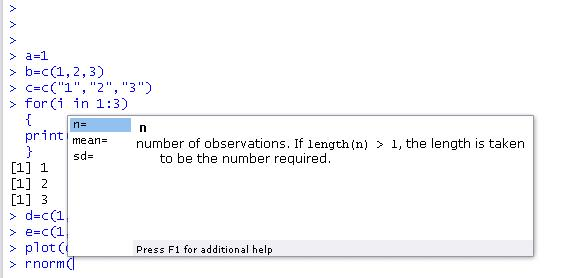
\includegraphics[width=10cm, clip=true, trim=0cm 0cm 0cm 1cm]{img/tab_RStudio.jpg}
  \caption{Το RStudio προτείνει πιθανά ορίσματα, εάν πατήσετε το \texttt{TAB} μετά από το όνομα της συνάρτησης
  και την παρένθεση.}
  \label{fig:tab_RStudio}
\end{figure*}

Πάλι για παράδειγμα, η συνάρτηση \texttt{rnorm} είναι μια πρότυπη συνάρτηση της R, η οποία δημιουργεί
τυχαία δείγματα από μία κανονική κατανομή. Πιέστε το πλήκτρο \texttt{ENTER} και θα δείτε 10 τυχαίους αριθμούς
όπως οι ακόλουθοι:

\begin{Verbatim}[frame=single,numbers=left,gobble=0, xleftmargin=0.35cm, numbersep=0.1cm]
> rnorm(10)
[1] -0.949  1.342 -0.474 0.403 
[5] -0.091 -0.379  1.015  0.740 
[9] -0.639  0.950
\end{Verbatim}

\noindent $\bullet$ Η γραμμή 1 περιέχει την εντολή: η \texttt{rnorm} είναι η συνάρτηση και το 10 είναι το όρισμα
που ορίζει πόσους τυχαίους αριθμούς επιθυμείτε --- σε αυτήν την περίπτωση, 10 αριθμούς (πληκτρολογώντας
\texttt{n=10} αντί μόνο του \texttt{10} θα δούλευε επίσης).\\
\noindent $\bullet$ Οι γραμμές 2-4 περιέχουν τα αποτελέσματα: 10 τυχαίους αριθμούς τοποθετημένους σε ένα
διάνυσμα μήκους 10.

Η εισαγωγή της ίδιας εντολής ξανά παράγει 10 νέους τυχαίους αριθμούς. Αντί να πληκτρολογήσετε το ίδιο κείμενο 
πάλι, μπορείτε επίσης να πιέσετε το πλήκτρο με το άνω βελάκι ($\uparrow$) για να προσπελάσετε παλιότερες 
εντολές. Εάν θέλετε 10 τυχαίους αριθμούς από μία κανονική κατανομή με μέσο όρο 1.2 και τυπική απόκλιση 3.4,
μπορείτε να πληκτρολογήσετε

\begin{Verbatim}[frame=single,gobble=0]
> rnorm(10, mean=1.2, sd=3.4)
\end{Verbatim}

κάτι που δείχνει ότι η ίδια συνάρτηση (\texttt{rnorm}) μπορεί να έχει διαφορετικές διεπαφές, και ότι η R έχει
τα λεγόμενα \emph{επώνυμα ορίσματα}  (σε αυτήν την περίπτωση τα \texttt{mean} και \texttt{sd}). Παρεμπιπτόντως,
τα κενά γύρω από το ``," και το ``=" δεν μετράνε.

Συγκρίνοντας αυτό το παράδειγμα με το προηγούμενο, βλέπει κανείς επίσης ότι για τη συνάρτηση \texttt{rnorm}
μόνο το πρώτο όρισμα (ο αριθμός 10) είναι υποχρεωτικό, και ότι η R δίνει προκαθορισμένες τιμές στα υπόλοιπα
προαιρετικά (όπως λέγονται) ορίσματα.\footnote{Χρησιμοποιήστε τη συνάρτηση help (ενότητα~\ref{sec:help}) για να
δείτε τις τιμές που χρησιμοποιούνται ως προκαθορισμένες.} 

Το RStudio έχει ένα ωραίο χαρακτηριστικό: εάν πληκτρολογήσετε \verb!rnorm(! στο παράθυρο εντολών και πιέσετε
\texttt{TAB}, τότε το RStudio θα εμφανίσει τα πιθανά ορίσματα (Σχήμα~\ref{fig:tab_RStudio}).

% ----- [05] Plots ---------------------------------------------------------------------------------------------
\subsection{Γραφικές παραστάσεις}

Η R μπορεί να φτιάξει γραφικές παραστάσεις. Το ακόλουθο είναι ένα πολύ απλό\footnote{Δείτε την ενότητα
~\ref{sec:some-plotting} για λίγο λιγότερο «ασήμαντα» παραδείγματα.} παράδειγμα:

\begin{Verbatim}[frame=single,numbers=left,gobble=0, xleftmargin=0.35cm, numbersep=0.1cm]
> x = rnorm(100)
> plot(x)
\end{Verbatim}

\noindent $\bullet$ Στην πρώτη γραμμή, εκχωρούνται 100 τυχαίοι αριθμοί στη μεταβλητή \texttt{x}, η οποία
γίνεται διάνυσμα μέσω αυτής της διαδικασίας. \\
\noindent $\bullet$ Στη δεύτερη γραμμή, όλες αυτές οι τιμές σχεδιάζονται στο παράθυρο γραφικών παραστάσεων.\\

\begin{ToDo}
Κάντε τη γραφική παράσταση 100 τυχαίων αριθμών (κανονικής κατανομής).\\
\end{ToDo}
% --------------------------------------------------------------------------------------------------------------


% --------------------------------------------------------------------------------------------------------------
% [#04] Help and documentation
% --------------------------------------------------------------------------------------------------------------
\section{Βοήθεια και τεκμηρίωση}
\label{sec:help}

Υπάρχει διαθέσιμο πολύ υλικό (δωρέαν) τεκμηρίωσης και βοήθειας. Ένα μέρος της βοήθειας εγκαθίσταται
αυτόματα. Η πληκτρολόγηση στο παράθυρο της κονσόλας της εντολής

\begin{Verbatim}[frame=single,gobble=0]
> help(rnorm)
\end{Verbatim}

θα σας προσφέρει βοήθεια σχετικά με την συνάρτηση \texttt{rnorm}. Σας δίνει μια περιγραφή της συνάρτησης,
πιθανά ορίσματα και τις τιμές που χρησιμοποιούνται ως προεπιλογή για τα προαιρετικά ορίσματα. Εάν
πληκτρολογήσετε

\begin{Verbatim}[frame=single,gobble=0]
> example(rnorm)
\end{Verbatim}

θα σας επιστρέψει μερικά παραδείγματα του πώς μπορεί να χρησιμοποιηθεί αυτή η συνάρτηση.

Καθολική βοήθεια βασισμένη σε HTML μπορεί να κληθεί μέσω της εντολής:

\begin{Verbatim}[frame=single,gobble=0]
> help.start()
\end{Verbatim}

ή με μετάβαση στο παράθυρο βοήθειας.

Οι ακόλουθοι σύνδεσμοι μπορεί επίσης να φανούν πολύ χρήσιμοι:\\
\noindent $\bullet$ \url{http://cran.r-project.org/doc/manuals/ R-intro.pdf} Ένα πλήρες εγχειρίδιο.\\
\noindent $\bullet$ \url{http://cran.r-project.org/doc/contrib/ Short-refcard.pdf} Μια σύντομη καρτέλα
αναφοράς.\\
\noindent $\bullet$  \url{http://zoonek2.free.fr/UNIX/48\_R/all.html}\\
Μια πολύ πλούσια πηγή παραδειγμάτων.\\
\noindent $\bullet$  \url{http://rwiki.sciviews.org/doku.php}\\
Ένα τυπικό wiki για χρήστες.\\
\noindent $\bullet$ \url{http://www.statmethods.net/}\\
Καλείται επίσης και Quick-R. Παρέχει πολύ παραγωγική και άμεση βοήθεια. Επίσης, κατάλληλη για χρήστες
που έρχονται από άλλες γλώσσες προγραμματισμού. \\
\noindent $\bullet$ \url{http://mathesaurus.sourceforge.net/}\\
Λεξικό για άλλες γλώσσες προγραμματισμού (π.χ. R για χρήστες Matlab). \\
\noindent $\bullet$  Και μόνο η χρήση της μηχανής Google (πληκτρολογήστε π.χ. ``R rnorm'' στο πεδίο αναζήτησης)
μπορεί να είναι πολύ παραγωγική.\\

\begin{ToDo}
Βρείτε βοήθεια για τη συνάρτηση \texttt{sqrt}.\\
\end{ToDo}
% --------------------------------------------------------------------------------------------------------------


% --------------------------------------------------------------------------------------------------------------
% [#05] Scripts
% --------------------------------------------------------------------------------------------------------------
\section{Σενάρια}

Η R είναι ένας διερμηνέας που χρησιμοποιεί ένα περιβάλλον βασισμένο στη γραμμή εντολών. Αυτό σημαίνει
ότι θα χρειαστεί να πληκτρολογείτε εντολές, αντί να χρησιμοποιείτε απλά το ποντίκι και τα μενού. Αυτό έχει
το πλεονέκτημα του ότι δε χρειάζεται εσείς να πληκτρολογείτε κάθε φορά ξανά όλες τις εντολές, και έτσι έχετε
λιγότερες πιθανότητες να εμφανίσετε πόνους στα χέρια, το λαιμό και τους ώμους σας.

Μπορείτε να αποθηκεύετε τις εντολές σας σε αρχεία, τα λεγόμενα \emph{σενάρια}. Αυτά τα σενάρια έχουν τυπικά
ονόματα αρχείων με την κατάληξη \texttt{.R}, π.χ. \texttt{foo.R}. Μπορείτε να ανοίξετε τον επεξεργαστή κειμένου
σε ένα παράθυρο και να επεξεργαστείτε αυτά τα αρχεία κάνοντας κλικ στο \texttt{File} και \texttt{New} ή στο 
\texttt{Open file...}\footnote{Όπου είναι διαθέσιμες επίσης και οι επιλογές \texttt{Save} και
\texttt{Save as}.}.

Μπορείτε να τρέξετε (να στείλετε δηλαδή στο παράθυρο κονσόλας) ένα μέρος του κώδικα, επιλέγοντας γραμμές του και
πατώντας \texttt{CTRL+ENTER} ή κάνοντας κλικ στο \texttt{Run} στο παράθυρο του επεξεργαστή κειμένου. Εάν δεν
επιλέξετε κάτι, η R θα τρέξει τη γραμμή στην οποία βρίσκεται ο κέρσορας. Μπορείτε πάντα να τρέξετε όλο το
σενάριο με την εντολή κονσόλας \texttt{source}, κι έτσι π.χ. για το σενάριο στο αρχείο \texttt{foo.R} θα πρέπει
να πληκτρολογήσετε:

\begin{Verbatim}[frame=single,gobble=0]
> source("foo.R")
\end{Verbatim}

Μπορείτε επίσης να κάνετε κλικ στο \texttt{Run all} στο παράθυρο του επεξεργαστή κειμένου ή να
πατήσετε τα πλήκτρα \texttt{CTRL+SHIFT+S} ώστε να τρέξετε ολόκληρο το σενάριο με τη μία.

\begin{ToDo}
Δημιουργήστε ένα αρχείο με όνομα \texttt{firstscript.R}, το οποίο θα περιέχει κώδικα R που θα δημιουργεί 100
τυχαίους αριθμούς και θα κάνει τη γραφική τους παράσταση, και τρέξτε αυτό το σενάριο αρκετές φορές.\\
\end{ToDo}
% --------------------------------------------------------------------------------------------------------------


% --------------------------------------------------------------------------------------------------------------
% [#06] Data structures
% --------------------------------------------------------------------------------------------------------------
\section{Δομές δεδομένων} 
\label{sec:structures}

Εάν δεν είστε αρκετά εξοικειωμένοι με την R, τότε είναι λογικό να επαναπληκτρολογείτε απλά τις εντολές που 
παρατίθενται σε αυτήν την ενότητα. Ίσως να μην χρειαστείτε όλες αυτές τις δομές στην αρχή, αλλά πάντα
είναι καλό να έχετε τουλάχιστον μια πρώτη εικόνα της ορολογίας και των πιθανών εφαρμογών.

% ----- [01] Vectors -------------------------------------------------------------------------------------------
\subsection{Διανύσματα}

Τα \emph{διανύσματα} τα έχουμε γνωρίσει ήδη, όμως μπορούν να κάνουν περισσότερα:

\begin{Verbatim}[frame=single,numbers=left,gobble=0, xleftmargin=0.35cm, numbersep=0.1cm]
> vec1 = c(1,4,6,8,10)
> vec1
[1]  1  4  6  8 10
> vec1[5]
[1] 10
> vec1[3] = 12
> vec1
[1]  1  4 12  8 10
> vec2 = seq(from=0, to=1, by=0.25)
> vec2
[1] 0.00 0.25 0.50 0.75 1.00
> sum(vec1)
[1] 35
> vec1 + vec2
[1]  1.00 4.25 12.50 8.75 11.00
\end{Verbatim}

\noindent $\bullet$  Στη γραμμή 1, ένα διάνυσμα \texttt{vec1} δημιουργείται ρητά από τη συνάρτηση συνένωσης
\texttt{c()}, την οποία έχουμε δει νωρίτερα. Τα στοιχεία των διανυσμάτων μπορούν να προσπελαστούν μέσω της
πρότυπης ευρετηρίασης \texttt{[i]}, όπως φαίνεται στις γραμμές 4-5. \\
\noindent $\bullet$  Στη γραμμή 6, ένα από τα στοιχεία αντικαθίσταται με ένα νέο αριθμό. Το αποτέλεσμα
εμφανίζεται στη γραμμή 8.\\
\noindent $\bullet$ Στη γραμμή 9 βλέπουμε ακόμα ένα χρήσιμο τρόπο δημιουργίας ενός διανύσματος: τη συνάρτηση
\texttt{seq()} (sequence ή ελληνιστί ακολουθία). \\
\noindent $\bullet$ Στις γραμμές 10-15 γίνονται μερικοί τυπικοί υπολογισμοί που αφορούν διανύσματα. Εάν
προσθέσετε δύο διανύσματα ίδιου μήκους, το πρώτο στοιχείο κάθε διανύσματος αθροίζεται με το άλλο, το ίδιο
και το δεύτερο, κ.ο.κ., έχοντας ως αποτέλεσμα ένα νέο διάνυσμα μήκους 5 (ακριβώς όπως και στους κανονικούς
υπολογισμούς με διανύσματα). Προσέξτε ότι η συνάρτηση \texttt{sum} αθροίζει όλα τα στοιχεία ενός διανύσματος,
έχοντας ως αποτέλεσμα έναν αριθμό (ένα βαθμωτό).

% ----- [02] Matrices ------------------------------------------------------------------------------------------
\subsection{Μητρώα}

Τα \emph{μητρώα} δεν είναι τίποτε άλλο παρά δισδιάστατα διανύσματα. Για να ορίσετε ένα μητρώο, χρησιμοποιήστε
τη συνάρτηση \texttt{matrix}:

\begin{Verbatim}[frame=single,numbers=left,gobble=0, xleftmargin=0.35cm, numbersep=0.1cm]
mat=matrix(data=c(9,2,3,4,5,6),ncol=3)
> mat
     [,1] [,2] [,3]
[1,]    9    3    5
[2,]    2    4    6
\end{Verbatim}

Το όρισμα \texttt{data} καθορίζει ποια νούμερα πρέπει να εισαχθούν στο μητρώο. Χρησιμοποιείστε είτε το 
\texttt{ncol} για να προσδιορίσετε τον αριθμό των στηλών, είτε το \texttt{nrow} για να προσδιορίσετε τον
αριθμό των γραμμών. 

\begin{ToDo}
Εισάγετε τους αριθμούς από το 31 έως το 60 σε ένα διάνυσμα με όνομα \texttt{P} και σε ένα μητρώο με 6 γραμμές
και 5 στήλες με όνομα \texttt{Q}. Υπόδειξη: χρησιμοποιείστε τη συνάρτηση \texttt{seq}. Δείτε τους διάφορους
τρόπους με τους οποίους συμβολίζονται οι βαθμωτοί, τα διανύσματα και τα μητρώα στο παράθυρο του χώρου 
εργασίας.\\
\end{ToDo}
 
Οι πράξεις με μητρώα είναι παρόμοιες με τις πράξεις σε διανύσματα:

\begin{Verbatim}[frame=single,numbers=left,gobble=0, xleftmargin=0.35cm, numbersep=0.1cm]
> mat[1,2]
[1] 3
> mat[2,]
[1] 2 4 6
> mean(mat)
[1] 4.8333
\end{Verbatim}

\noindent $\bullet$ Τα στοιχεία ενός μητρώου μπορούν να προσπελαστούν με το συνήθη τρόπο: \texttt{[row,column]}
(γραμμή 1). \\
\noindent $\bullet$ Γραμμή 3: όταν θελήσετε να επιλέξετε μια ολόκληρη γραμμή, αφήστε τη θέση για το όρισμα του
αριθμού των στηλών κενή (και φυσικά το ανάποδο όταν θελήσετε στήλες).\\
\noindent $\bullet$ Στη γραμμή 5 βλέπουμε ότι πολλές συναρτήσεις εξακολουθούν να δουλεύουν όταν έχουν μητρώα
ως όρισμα.\\

% ----- [03] Data frames ---------------------------------------------------------------------------------------
\subsection{Πλαίσια δεδομένων}

Οι χρονοσειρές (time series) συχνά κατατάσσονται στα \emph{πλαίσια δεδομένων} (data frames). Ένα πλαίσιο
δεδομένων είναι ένα μητρώο με ονόματα πάνω από τις στήλες του. Αυτό είναι καλό, γιατί έτσι μπορείτε να καλέσετε
και να χρησιμοποιήσετε όποια από τις στήλες θέλετε χωρίς να γνωρίζετε σε ποια θέση είναι αυτή.

\begin{Verbatim}[frame=single,numbers=left,gobble=0, xleftmargin=0.35cm, numbersep=0.1cm]
> t = data.frame(x = c(11,12,14),
 y = c(19,20,21), z = c(10,9,7))
> t
   x y z
1 11 19 10
2 12 20 9 
3 14 21 7  
> mean(t$z)
[1] 8.666667
> mean(t[["z"]])
[1] 8.666667
\end{Verbatim}
%%$

\noindent $\bullet$ Στις γραμμές 1-2 κατασκευάζεται ένα τυπικό πλαίσιο δεδομένων με όνομα \texttt{t}. Οι στήλες
έχουν τα ονόματα \texttt{x}, \texttt{y} and \texttt{z}.\\
\noindent $\bullet$ Στις γραμμές 8-11 βλέπουμε δύο τρόπους με τους οποίους μπορείτε να επιλέξετε τη στήλη με 
όνομα \texttt{z} από το πλαίσιο δεδομένων με όνομα \texttt{t}.\\
\\

\begin{ToDo}
Δημιουργήστε ένα σενάριο το οποίο θα κατασκευάζει τρία τυχαία (κανονικά) διανύσματα μήκους 100. Ονομάστε
αυτά τα διανύσματα \texttt{x1}, \texttt{x2} και \texttt{x3}. Φτιάξτε ένα πλαίσιο δεδομένων με όνομα \texttt{t}
με τρεις στήλες (που θα λέγονται \texttt{a}, \texttt{b} και \texttt{c}) που θα περιέχει αντίστοιχα τα 
\texttt{x1}, \texttt{x1+x2} και \texttt{x1+x2+x3}. Καλέστε τις ακόλουθες συναρτήσεις για αυτό το πλαίσιο
δεδομένων: \texttt{plot(t)} και \texttt{sd(t\$x1)}. Μπορείτε να κατανοήσετε τα αποτελέσματα; Τρέξτε το
σενάριο ξανά μερικές φορές.\\
\end{ToDo}

% ----- [04] Lists ---------------------------------------------------------------------------------------------
\subsection{Λίστες}

Μια άλλη βασική δομή στην R είναι η \emph{λίστα}. Το κύριο πλεονέκτημα των λιστών είναι ότι οι «στήλες»
(δεν είναι πλέον διατεταγμένες σε στήλες, αλλά μοιάζουν πιο πολύ με μια συλλογή διανυσμάτων) δεν είναι
υποχρεωτικό να έχουν το ίδιο μήκος, αντίθετα με τις περιπτώσεις των μητρώων και των πλαισίων δεδομένων.

\begin{Verbatim}[frame=single,numbers=left,gobble=0, xleftmargin=0.35cm, numbersep=0.1cm]
> L = list(one=1, two=c(1,2), 
 five=seq(0, 1, length=5))
> L
$one
[1] 1
$two
[1] 1 2
$five
[1] 0.00 0.25 0.50 0.75 1.00
> names(L)
[1] "one"  "two"  "five"
> L$five + 10
[1] 10.00 10.25 10.50 10.75 11.00
\end{Verbatim}

\noindent $\bullet$ Στις γραμμές 1-2 δημιουργείται μια λίστα μέσω της εισόδου ονομάτων και τιμών. Η λίστα
εμφανίζεται επίσης και στο παράθυρο του χώρου εργασίας.\\
\noindent $\bullet$ Στις γραμμές 3-9 φαίνεται μια τυπική εκτύπωση (μετά από πάτημα των \texttt{L} και
\texttt{ENTER}). \\
\noindent $\bullet$ Η γραμμή 10 δείχνει πώς μπορούμε να δούμε τι υπάρχει μέσα στη λίστα.\\
\noindent $\bullet$ Η γραμμή 12 παρουσιάζει έναν τρόπο χρήσης των αριθμών. \\
% --------------------------------------------------------------------------------------------------------------


% --------------------------------------------------------------------------------------------------------------
% [#07] Graphics
% --------------------------------------------------------------------------------------------------------------
\section{Γραφικά}
\label{sec:some-plotting}

Η σχεδίαση γραφικών παραστάσεων είναι μια σημαντική στατιστική δραστηριότητα. Οπότε δεν πρέπει να σας εκπλήσσει
το γεγονός ότι η R έχει πολλές δυνατότητες σχεδιασμού γραφικών παραστάσεων. Οι ακόλουθες γραμμές εμφανίζουν ένα
απλό γράφημα:

\begin{Verbatim}[frame=single,gobble=0]
> plot(rnorm(100), type="l", col="gold")
\end{Verbatim}

\noindent Εκατοντάδες τυχαίοι αριθμοί αναπαρίστανται γραφικά μέσω της σύνδεσης των σημείων με γραμμές (το 
σύμβολο μέσα σε εισαγωγικά μετά το \texttt{type=} είναι το γράμμα l, όχι ο αριθμός 1) σε χρυσό χρώμα.

Ένα άλλο πολύ απλό παράδειγμα είναι το κλασικό στατιστικό γράφημα του ιστογράμματος, που δημιουργείται από
την απλή εντολή

\begin{Verbatim}[frame=single,gobble=0]
  > hist(rnorm(100))
\end{Verbatim}

η οποία παράγει το γράφημα στο Σχήμα~\ref{fig:hist}.

\begin{figure}[h]
  \centering
  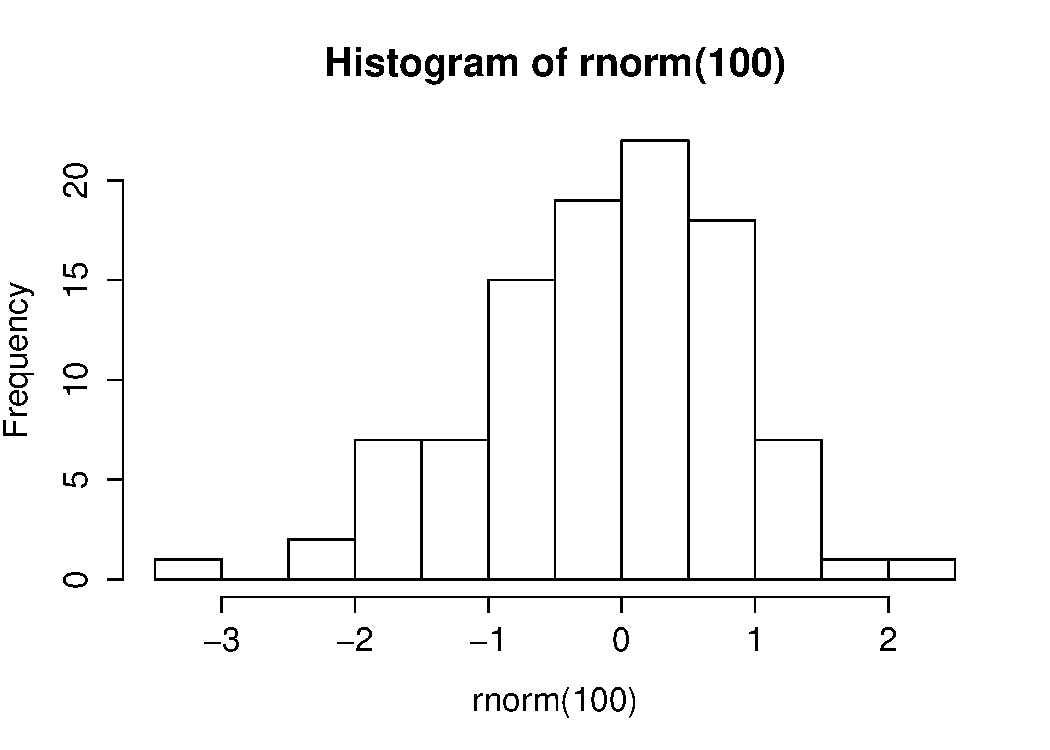
\includegraphics[width=8cm]{img/hist.pdf}
  \caption{Ένα απλό ιστόγραμμα.}
  \label{fig:hist}
\end{figure}

\noindent Οι ακόλουθες γραμμές δημιουργούν ένα γράφημα χρησιμοποιώντας το πλαίσιο δεδομένων \texttt{t} που 
φτιάξαμε στο προηγούμενο ToDo:

\begin{Verbatim}[frame=single,numbers=left,gobble=0, xleftmargin=0.35cm, numbersep=0.1cm]
plot(t$a, type="l", ylim=range(t), 
 lwd=3, col=rgb(1,0,0,0.3))
lines(t$b, type="s", lwd=2, 
 col=rgb(0.3,0.4,0.3,0.9))
points(t$c, pch=20, cex=4, 
 col=rgb(0,0,1,0.3))
\end{Verbatim} 
%%$ 

\begin{ToDo}
Προσθέστε αυτές τις γραμμές στο αρχείο σεναρίου της προηγούμενης ενότητας. Δοκιμάστε να ανακαλύψετε, είτε 
μέσω πειραματισμών, είτε με τη χρήση της βοήθειας, ποιο είναι το νόημα της \texttt{rgb}, του τελευταίου
ορίσματος της \texttt{rgb}, του \texttt{lwd}, του \texttt{pch}, και του \texttt{cex}.\\
\end{ToDo}

Για να μάθετε περισσότερα σχετικά με τη μορφοποίηση των γραφημάτων, ψάξτε το \texttt{par} στη βοήθεια της R.
Κάντε αναζήτηση στη μηχανή της Google τον όρο ``R color chart" για να βρείτε ένα αρχείο pdf που περιέχει
πληθώρα επιλογών χρωμάτων.

Για να αντιγράψετε τη γραφική σας παράσταση σε ένα έγγραφο, πηγαίνετε στο παράθυρο των γραφικών παραστάσεων,
κάντε κλικ στο κουμπί ``Export", επιλέξτε το μήκος και πλάτος που σας αρέσει περισσότερο και κάντε κλικ στο
\texttt{Copy} ή στο \texttt{Save}. 
% --------------------------------------------------------------------------------------------------------------


% --------------------------------------------------------------------------------------------------------------
% [#08] Reading and writing data files
% --------------------------------------------------------------------------------------------------------------
\section{Διαβάζοντας από και γράφοντας σε αρχεία δεδομένων}
\label{sec:reading-writing-data}

Υπάρχουν πολλοί τρόποι για να καταγράψει κανείς δεδομένα σε αρχεία μέσω του περιβάλλοντος της R, και για να 
διαβάσει δεδομένα από αρχεία. Εδώ θα παρουσιάσουμε έναν τέτοιο τρόπο. Οι ακόλουθες γραμμές παρουσιάζουν τα
στοιχειώδη:

\begin{Verbatim}[frame=single,numbers=left,gobble=0, xleftmargin=0.35cm, numbersep=0.1cm]
> d = data.frame(a = c(3,4,5), 
 b = c(12,43,54))
> d
  a  b
1 3 12
2 4 43
3 5 54
> write.table(d, file="tst0.txt",
 row.names=FALSE)
> d2 = read.table(file="tst0.txt", 
 header=TRUE)
> d2
  a  b
1 3 12
2 4 43
3 5 54
\end{Verbatim}

\noindent $\bullet$ Στις γραμμές 1-2, δημιουργείται ένα απλό πλαίσιο δεδομένων ως παράδειγμα και αποθηκεύεται 
στη μεταβλητή \texttt{d}. \\
\noindent $\bullet$ Στις γραμμές 3-7 φαίνεται το περιεχόμενο αυτού του πλαισίου δεδομένων: δύο στήλες (με 
όνομα \texttt{a} και \texttt{b}), κάθε μία από τις οποίες περιέχει τρεις αριθμούς.\\
\noindent $\bullet$ Στη γραμμή 8 καταγράφεται αυτό το πλαίσιο δεδομένων σε ένα αρχείο κειμένου, με όνομα
\texttt{tst0.txt} Το όρισμα \verb!row.names=FALSE! αποτρέπει τα ονόματα των γραμμών να καταγραφούν στο αρχείο.
Επειδή δεν καθορίζεται κάτι για τα \texttt{col.names} (ονόματα των στηλών), επιλέγεται η προκαθορισμένη επιλογή
\verb!col.names=TRUE! και τα ονόματα των στηλών καταγράφονται στο αρχείο. Στο Σχήμα~\ref{fig:tst0} φαίνεται το
τελικό αρχείο (ανοιγμένο σε έναν επεξεργαστή κειμένου, όπως το Σημειωματάριο), με τα ονόματα των στηλών
(\texttt{a} και \texttt{b})στην πρώτη γραμμή. \\
\noindent $\bullet$ Οι γραμμές 10-11 δείχνουν πώς μπορούμε να εισάγουμε ένα αρχείο μέσα σε ένα πλαίσιο
δεδομένων. Σημειώστε ότι εισάγονται και τα ονόματα των στηλών. Το πλαίσιο δεδομένων εμφανίζεται επίσης στο
παράθυρο του χώρου εργασίας.\\

\begin{figure}[h]
  \centering
  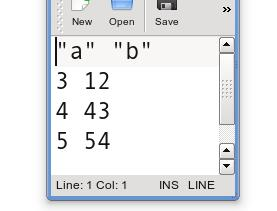
\includegraphics[width=3.5cm]{img/tst0.jpeg}
  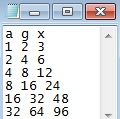
\includegraphics[width=2.6cm]{img/tst1.jpg}
  \caption{Τα αρχεία \texttt{tst0.txt} της ενότητας~\ref{sec:reading-writing-data}
    (αριστερά) και \texttt{tst1.txt} από το ToDo παρακάτω (δεξιά), ανοιγμένα σε δύο επεξεργαστές κειμένου.}
  \label{fig:tst0}
\end{figure}

\begin{ToDo}
Φτιάξτε ένα αρχείο με όνομα \texttt{tst1.txt} στο Σημειωματάριο από το παράδειγμα του Σχήματος~\ref{fig:tst0}
και αποθηκεύστε το στον κατάλογο εργασίας σας. Γράψτε ένα σενάριο που να το διαβάζει, που να πολλαπλασιάζει
τη στήλη με όνομα \texttt{g} επί 5 και να την αποθηκεύει με όνομα \texttt{tst2.txt}.\\
\end{ToDo}
% --------------------------------------------------------------------------------------------------------------


% --------------------------------------------------------------------------------------------------------------
% [#09] Not available data
% --------------------------------------------------------------------------------------------------------------
\section{Μη-διαθέσιμα δεδομένα}

\begin{ToDo}
Υπολογίστε το μέσο όρο της τετραγωνικής ρίζας ενός διανύσματος 100 τυχαίων αριθμών. Τι θα συμβεί;
\end{ToDo}

Όταν δουλεύετε με πραγματικά δεδομένα, θα βρεθείτε αντιμέτωποι με τιμές που λείπουν επειδή υπήρξαν αστοχίες
στα όργανα μέτρησης ή επειδή δεν θέλατε να κάνετε μετρήσεις το Σαββατοκύριακο. Όταν ένα δεδομένο \emph{δεν
είναι διαθέσιμο}, τότε πρέπει να γράψετε \texttt{NA} (τα αρχικά του ``Not Available") αντί κάποιου αριθμού. 

\begin{Verbatim}[frame=single,gobble=0]
> j = c(1,2,NA)
\end{Verbatim}

Ο υπολογισμός στατιστικών από ημιτελή σύνολα δεδομένων είναι αδύνατος, αυστηρά μιλώντας. Μπορεί η μέγιστη τιμή
να εμφανίστηκε κατά τη διάρκεια του Σαββατοκύριακου, όταν δεν κάνατε μετρήσεις. Κατά συνέπεια, η R θα σας πει
ότι δε γνωρίζει ποια είναι η μέγιστη τιμή του \texttt{j}: 

\begin{Verbatim}[frame=single,gobble=0]
> max(j)
[1] NA
\end{Verbatim}

Εάν δεν έχετε πρόβλημα με τα δεδομένα που λείπουν και θέλετε να υπολογίσετε τα στατιστικά όπως και να 'χει,
μπορείτε να προσθέσετε το όρισμα \texttt{na.rm=TRUE} (να απομακρύνω/remove/rm τις τιμές NA; Ναι!). 

\begin{Verbatim}[frame=single,gobble=0]
> max(j, na.rm=TRUE)
[1] 2
\end{Verbatim}
% --------------------------------------------------------------------------------------------------------------


% --------------------------------------------------------------------------------------------------------------
% [#10] Classes
% --------------------------------------------------------------------------------------------------------------
\section{Κλάσεις}

Οι ασκήσεις που κάνατε πριν ήταν σχεδόν όλες με αριθμούς. Μερικές φορές θα χρειαστεί να προσδιορίσετε κάτι το 
οποίο δεν είναι αριθμός, για παράδειγμα το όνομα ενός σταθμού μετρήσεων ή ενός αρχείου δεδομένων. Σε αυτήν την
περίπτωση θέλετε η μεταβλητή να είναι μια ακολουθία χαρακτήρων αντί να είναι αριθμός. 

Ένα αντικείμενο στην R μπορεί να έχει διάφορες από τις λεγόμενες \emph{κλάσεις}. Οι τρεις πιο σημαντικές είναι
η \emph{numeric}, η \emph{character} και η \emph{POSIX} (συνδυασμοί ημερομηνίας-ώρας). Μπορείτε να ρωτήσετε
την R ποια είναι η κλάση μιας συγκεκριμένης μεταβλητής πληκτρολογώντας \texttt{class(...)}. 

% ----- [01] Characters ----------------------------------------------------------------------------------------
\subsection{Χαρακτήρες}
\label{sec:characters}

Για να δηλώσετε στην R ότι κάτι είναι ακολουθία χαρακτήρων, πρέπει να πληκτρολογήσετε το κείμενο ανάμεσα σε
αποστρόφους, αλλιώς η R θα αρχίσει να ψάχνει για μια καθορισμένη μεταβλητή με το ίδιο όνομα:

\begin{Verbatim}[frame=single,gobble=0]
> m = "apples"
> m
[1] "apples"
> n = pears
Error: object `pears' not found
\end{Verbatim}

Φυσικά, δεν μπορείτε να κάνετε υπολογισμούς με ακολουθίες χαρακτήρων:

\begin{Verbatim}[frame=single,gobble=0]
> m + 2
Error in m + 2 : non-numeric argument to 
binary operator
\end{Verbatim}

% ----- [02] Dates ---------------------------------------------------------------------------------------------
\subsection{Ημερομηνίες}

Οι ημερομηνίες και οι ώρες είναι πολύπλοκες περιπτώσεις. Η R πρέπει να να γνωρίζει ότι η ώρα 3 ακριβώς είναι
μετά από τις 2:59 και ότι ο Φεβρουάριος έχει 29 ημέρες σε μερικά έτη. Ο ευκολότερος τρόπος για να πείτε
στην R ότι κάτι αποτελεί συνδυασμό ημερομηνίας-ώρας είναι μέσω της συνάρτησης \texttt{strptime}:

\begin{Verbatim}[frame=single,numbers=left,gobble=0, xleftmargin=0.35cm, numbersep=0.1cm]
> date1=strptime( c("20100225230000", 
 "20100226000000", "20100226010000"), 
 format="%Y%m%d%H%M%S")
 > date1
[1] "2010-02-25 23:00:00" 
[2] "2010-02-26 00:00:00" 
[3] "2010-02-26 01:00:00"
\end{Verbatim}

\noindent $\bullet$  Στις γραμμές 1-2 δημιουργείται ένα διάνυσμα με την \texttt{c(...)}. Οι αριθμοί στα 
διανύσματα είναι ανάμεσα σε αποστρόφους, επειδή η συνάρτηση \texttt{strptime} απαιτεί ακολουθίες χαρακτήρων ως
είσοδο.\\
\noindent $\bullet$ Στη γραμμή 3 το όρισμα \texttt{format} προσδιορίζει πώς θα πρέπει να διαβαστεί η ακολουθία
χαρακτήρων. Σε αυτή την περίπτωση το έτος αναπαρίσταται στην αρχή (\%Y), έπειτα ο μήνας (\%m), η ημέρα (\%d),
η ώρα (\%H), τα λεπτά (\%M) και τα δευτερόλεπτα (\%S). Δεν χρειάζεται να τα προσδιορίσετε όλα αυτά, εφόσον η
μορφή αυτή είναι αντίστοιχη με την ακολουθία εισόδου.

\begin{ToDo}
Δημιουργήστε ένα γράφημα, το οποίο θα έχει στον άξονα των x ημερομηνίες από τις 6 Δεκεμβρίου 2014 έως τα επόμενα 
γενέθλιά σας, και στον άξονα των y τον αριθμό των δώρων που περιμένετε σε κάθε μία από αυτές τις μέρες.
Υπόδειξη: φτιάξτε δύο διανύσματα πρώτα.
\end{ToDo}
% --------------------------------------------------------------------------------------------------------------


% --------------------------------------------------------------------------------------------------------------
% [#11] Programming tools
% --------------------------------------------------------------------------------------------------------------
\section{Προγραμματιστικά εργαλεία}

Όταν φτιάχνετε ένα μεγαλύτερο πρόγραμμα από τα προηγούμενα παραδείγματα ή όταν χρησιμοποιείτε τα σενάρια κάποιου
άλλου, μπορεί να συναντήσετε κάποιες προγραμματιστικές δομές. Στην ενότητα αυτή θα περιγράψουμε μερικές
σχετικές συμβουλές και κόλπα.

% ----- [01] If-statement --------------------------------------------------------------------------------------
\subsection{Δομή ελέγχου if}

Η δομή ελέγχου \emph{if} χρησιμοποιείται όταν συγκεκριμένοι υπολογισμοί πρέπει να γίνουν \emph{μόνο} όταν
ικανοποιείται μια συγκεκριμένη συνθήκη (και πιθανόν να πρέπει να γίνει κάτι άλλο, όταν η συνθήκη δεν
ικανοποιείται). Ένα παράδειγμα:

\begin{Verbatim}[frame=single,numbers=left,gobble=0, xleftmargin=0.35cm, numbersep=0.1cm]
> w = 3
> if( w < 5 )
   {
   d=2
   }else{
   d=10
   }
> d
2
\end{Verbatim}

\noindent $\bullet$ Στη γραμμή 2 καθορίζεται μια συνθήκη: το \texttt{w} πρέπει να είναι μικρότερο του 5.\\
\noindent $\bullet$ Εάν η συνθήκη ικανοποιηθεί, τότε η R θα εκτελέσει ό,τι βρίσκεται ανάμεσα στις πρώτες αγκύλες
στη γραμμή 4.\\
\noindent $\bullet$ Εάν η συνθήκη \emph{δεν} ικανοποιηθεί, τότε η R θα εκτελέσει ό,τι βρίσκεται ανάμεσα στις
δεύτερες αγκύλες, μετά το \texttt{else} στης γραμμή 6. Μπορείτε να παραλείψετε το κομμάτι του \verb!else{...}!
εάν δεν το χρειάζεστε.\\
\noindent $\bullet$ Σε αυτή την περίπτωση, η συνθήκη ικανοποιείται και στη μεταβλητή \texttt{d} εκχωρείται
η τιμή 2 (γραμμές 8-9).

Για να πάρετε ένα υποσύνολο στοιχείων ενός διανύσματος για τα οποία ισχύει μια συγκεκριμένη συνθήκη, μπορείτε 
να χρησιμοποιήσετε μια πιο σύντομη μέθοδο:

\begin{Verbatim}[frame=single,numbers=left,gobble=0, xleftmargin=0.35cm, numbersep=0.1cm]
> a = c(1,2,3,4)
> b = c(5,6,7,8)
> f = a[b==5 | b==8]
> f
[1] 1 4
\end{Verbatim}

\noindent $\bullet$ Στη γραμμή 1 και 2 δημιουργούνται δύο διανύσματα.\\
\noindent $\bullet$ Στη γραμμή 3 δηλώνετε ότι η \texttt{f} συντίθεται από εκείνα τα στοιχεία του διανύσματος
\texttt{a} για τα οποία τα αντίστοιχα στοιχεία του \texttt{b} ισούται με 5 ή με 8. \\

Προσέξτε το διπλό \texttt{=} στη συνθήκη. Άλλες συνθήκες (που ονομάζονται επίσης λογικοί ή Boolean τελεστές)
είναι οι \texttt{<}, \texttt{>}, \texttt{!=} ($\neq$), \texttt{<=} ($\leq$) και \texttt{>=} ($\geq$). Για να
ελέγξετε περισσότερες από μία συνθήκες σε μία δομή if, χρησιμοποιήστε το \texttt{\&} εάν και οι δύο 
συνθήκες πρέπει να ικανοποιούνται (λογικό «και» - ``and") και το \texttt{|} εάν μία από τις συνθήκες πρέπει να 
ικανοποιείται (λογικό «ή» - ``or").

% ----- [02] For-loop ------------------------------------------------------------------------------------------
\subsection{Βρόχος επανάληψης for}

Όταν θέλετε να μοντελοποιήσετε μια χρονοσειρά, συνήθως κάνετε τους υπολογισμούς για ένα χρονικό βήμα και έπειτα
για το επόμενο και για το μεθεπόμενο, κ.ο.κ. Επειδή κανένας δε θέλει να πληκτρολογεί τις ίδιες εντολές ξανά
και ξανά, αυτοί οι υπολογισμοί μπορούν να αυτοματοποιηθούν με βρόχους επανάληψης for.

Σε έναν \emph{βρόχο for} προσδιορίζετε τι πρέπει να γίνει και πόσες φορές πρέπει να γίνει. Για να δηλώσετε το 
«πόσες φορές», καθορίζετε το λεγόμενο μετρητή. Ένα παράδειγμα:

\begin{Verbatim}[frame=single,numbers=left,gobble=0, xleftmargin=0.35cm, numbersep=0.1cm]
> h = seq(from=1, to=8)
> s = c()
> for(i in 2:10) 
   {
   s[i] = h[i] * 10
   }
> s
[1] NA 20 30 40 50 60 70 80 NA NA
\end{Verbatim}

\noindent $\bullet$ Αρχικά δημιουργείται το διάνυσμα \texttt{h}.\\
\noindent $\bullet$ Στη γραμμή 2 δημιουργείται ένα κενό διάνυσμα (\texttt{s}). Αυτό είναι απαραίτητο γιατί όταν
δημιουργείτε μια μεταβλητή μέσα σε βρόχο for, η R δε θα είναι σε θέση να τη θυμάται όταν βγει έξω από αυτόν.\\
\noindent $\bullet$  Στη γραμμή 3 ξεκινάει ο βρόχος for. Σε αυτή την περίπτωση, το \texttt{i} είναι ο μετρητής
και τρέχει από το 2 έως το 10.\\
\noindent $\bullet$ Οτιδήποτε βρίσκεται ανάμεσα στις αγκύλες (γραμμή 5) θα υποστεί επεξεργασία 9 φορές. Την
πρώτη φορά για \texttt{i=2}, το δεύτερο στοιχείο του \texttt{h} πολλαπλασιάζεται με 10 και τοποθετείται στη
δεύτερη θέση του διανύσματος \texttt{s}. Την δεύτερη φορά για \texttt{i=3}, κτλ. Στις τελευταίες δύο εκτελέσεις,
ζητούνται το 9\textsuperscript{ο} και 10\textsuperscript{ο} στοιχείο του \texttt{h}, τα οποία δεν υπάρχουν.
Σημειώστε ότι αυτές οι δηλώσεις ελέγχονται και υπολογίζονται χωρίς να υπάρχει κάποιο ρητό μήνυμα λάθους.

\begin{ToDo}
Δημιουργήστε ένα διάνυσμα από το 1 έως το 100. Φτιάξτε ένα βρόχο for ο οποίος θα διατρέχει ολόκληρο το διάνυσμα.
Πολλαπλασιάστε τα στοιχεία τα οποία είναι μικρότερα του 5 και μεγαλύτερα του 90 επί 10, και τα υπόλοιπα στοιχεία
επί 0.1.
\end{ToDo}

% ----- [03] Writing your own functions ------------------------------------------------------------------------
\subsection{Γράφοντας τις δικές σας συναρτήσεις}
\label{sec:progfunc}

Οι συναρτήσεις που προγραμματίζετε εσείς οι ίδιοι λειτουργούν με τον ίδιο τρόπο που λειτουργούν οι συναρτήσεις
που είναι προ-προγραμματισμένες μέσα στην R.

\begin{Verbatim}[frame=single,numbers=left,gobble=0, xleftmargin=0.35cm, numbersep=0.1cm]
> fun1 = function(arg1, arg2 )
   {
   w = arg1 ^ 2
   return(arg2 + w)
   }
> fun1(arg1 = 3, arg2 = 5) 
[1] 14

\end{Verbatim}

\noindent $\bullet$ Στη γραμμή 1 καθορίζεται το όνομα της συνάρτησης (\texttt{fun1}) και τα ορίσματά της
(\texttt{arg1} και \texttt{arg2}). \\
\noindent $\bullet$ Στις γραμμές 2-5 καθορίζεται το τι θα πρέπει να κάνει η συνάρτηση όταν καλεστεί. Η τιμή
που θα επιστρέφει (\texttt{arg2+w}) εμφανίζεται στην οθόνη. \\
\noindent $\bullet$ Στη γραμμή 6 καλείται η συνάρτηση με ορίσματα 3 και 5.

\begin{ToDo}
Γράψτε μια συνάρτηση για το προηγούμενο ToDo, ώστε να μπορείτε να την τροφοδοτείτε με οποιοδήποτε διάνυσμα 
επιθυμείτε εσείς (ως όρισμα). Χρησιμοποιήστε ένα βρόχο for μέσα στη συνάρτηση ώστε να κάνετε τον υπολογισμό
κάθε στοιχείου. Χρησιμοποιείστε την πρότυπη συνάρτηση της R \texttt{length} κατά τον προσδιορισμό του μετρητή.
\footnote{Στην πραγματικότητα, οι χρήστες χρησιμοποιούν πιο συχνά βρόχους for απ' ότι είναι ουσιαστικά
απαραίτητο. Το παραπάνω ToDo μπορεί να γίνει πιο εύκολα και γρήγορα χωρίς τη χρήση βρόχου for, μα με 
τυπικούς υπολογισμούς διανυσμάτων.})
\end{ToDo}
% --------------------------------------------------------------------------------------------------------------


% --------------------------------------------------------------------------------------------------------------
% [#12] Some useful references
% --------------------------------------------------------------------------------------------------------------
\section{Μερικές χρήσιμες αναφορές}

% ----- [01] Functions -----------------------------------------------------------------------------------------
\subsection{Συναρτήσεις}

Το παρακάτω είναι ένα υποσύνολο από συναρτήσεις που επεξηγούνται στην καρτέλα αναφορών (reference card) της R.\\

\noindent \underline{Δημιουργία δεδομένων (data creation)}\vspace{0.2cm}\\
$\bullet$ \texttt{read.table}: διάβασε έναν πίνακα από ένα αρχείο. Ορίσματα: \texttt{header=TRUE}: διάβασε
την πρώτη γραμμή ως τίτλους των στηλών\anoteleia \texttt{sep=","}: οι αριθμοί διαχωρίζονται με κόμμα\anoteleia
\texttt{skip=n}: μη διαβάσεις τις πρώτες \texttt{n} γραμμές.\\
$\bullet$ \texttt{write.table}: αποθήκευσε έναν πίνακα σε ένα αρχείο\\
$\bullet$ \texttt{c}: συνένωσε αριθμούς μεταξύ τους ώστε να δημιουργήσεις ένα διάνυσμα\\
$\bullet$ \texttt{array}: δημιούργησε ένα διάνυσμα, Ορίσματα: \texttt{dim}: μήκος\\
$\bullet$ \texttt{matrix}: δημιούργησε ένα μητρώο, Ορίσματα: \texttt{ncol} και/ή \texttt{nrow}: αριθμός γραμμών/
στηλών\\
$\bullet$ \texttt{data.frame}: δημιούργησε ένα πλαίσιο δεδομένων\\
$\bullet$ \texttt{list}: δημιούργησε μια λίστα\\
$\bullet$ \texttt{rbind} και \texttt{cbind}: συνένωσε διανύσματα σε ένα μητρώο κατά γραμμή ή κατά στήλη\\

\noindent \underline{Εξαγωγή δεδομένων (extracting data)}\vspace{0.2cm}\\
$\bullet$ \texttt{x[n]}: το \texttt{n}-στο στοιχείο ενός διανύσματος\\
$\bullet$ \texttt{x[m:n]}: από το \texttt{m}-στο έως το \texttt{n}-στο στοιχείο\\
$\bullet$ \texttt{x[c(k,m,n)]}: συγκεκριμένα στοιχεία\\
$\bullet$ \texttt{x[x>m \& x<n]}: τα στοιχεία ανάμεσα στο \texttt{m} και \texttt{n}\\
$\bullet$ \verb!x$n!:  το στοιχείο της λίστας ή του πλαισίου δεδομένων με όνομα \texttt{n}\\
$\bullet$ \texttt{x[["n"]]}: ό.π.\\
$\bullet$ \texttt{[i,j]}: το στοιχείο στην \texttt{i}-στη γραμμή και \texttt{j}-στη στήλη \\
$\bullet$ \texttt{[i,]}: η γραμμή \texttt{i} σε ένα μητρώο\\

\noindent \underline{Πληροφορίες για μεταβλητές}\vspace{0.2cm}\\
$\bullet$ \texttt{length}: το μήκος ενός διανύσματος\\
$\bullet$ \texttt{ncol} ή \texttt{nrow}: ο αριθμός των στηλών ή των γραμμών ενός μητρώου\\
$\bullet$ \texttt{class}: η κλάση μιας μεταβλητής \\
$\bullet$ \texttt{names}: τα ονόματα των αντικειμένων σε μια λίστα \\
$\bullet$ \texttt{print}: εμφάνισε τη μεταβλητή ή την ακολουθία χαρακτήρων στην οθόνη (χρησιμοποιείται σε
σενάρια ή σε βρόχους for) \\
$\bullet$ \texttt{return}: εμφάνισε τη μεταβλητή στην οθόνη (χρησιμοποιείται σε συναρτήσεις) \\
$\bullet$ \texttt{is.na}: έλεγξε εάν η μεταβλητή ισούται με \texttt{NA}\\
$\bullet$ \texttt{as.numeric} ή \texttt{as.character}: άλλαξε την κλάση σε αριθμό ή σε ακολουθία γραμμάτων\\
$\bullet$ \texttt{strptime}: άλλαξε την κλάση από χαρακτήρα σε ημερομηνία-ώρα (POSIX)\\

\noindent \underline{Στατιστικά}\vspace{0.2cm}\\
$\bullet$ \texttt{sum}: το άθροισμα ενός διανύσματος (ή ενός μητρώου)\\
$\bullet$ \texttt{mean}: ο μέσος όρος ενός διανύσματος\\
$\bullet$ \texttt{sd}: η τυπική απόκλιση ενός διανύσματος\\
$\bullet$ \texttt{max} ή \texttt{min}: μέγιστο ή ελάχιστο στοιχείο\\
$\bullet$ \texttt{rowSums} (ή \texttt{rowMeans}, \texttt{colSums} και \texttt{colMeans}): 
αθροίσματα (ή μέσοι όροι) όλων των αριθμών σε κάθε γραμμή (ή στήλη) ενός μητρώου. Το αποτέλεσμα είναι ένα
διάνυσμα.\\
$\bullet$ \texttt{quantile(x,c(0.1,0.5))}: δειγματοληψία του 0.1-στου και του 0.5-στου ποσοστημόριου του
διανύσματος \texttt{x}\\

\noindent \underline{Επεξεργασία δεδομένων}\vspace{0.2cm}\\
$\bullet$ \texttt{seq}: δημιούργησε ένα διάνυσμα με ίσες αποστάσεις μεταξύ των αριθμών\\
$\bullet$ \texttt{rnorm}: δημιούργησε ένα διάνυσμα με τυχαίους αριθμούς που ακολουθούν την κανονική κατανομή
(και άλλες κατανομές είναι επίσης διαθέσιμες)\\
$\bullet$ \texttt{sort}: ταξινόμησε τα στοιχεία σε αύξουσα διάταξη\\
$\bullet$ \texttt{t}: αντίστρεψε ένα μητρώο\\
$\bullet$ \texttt{aggregate(x,by=ls(y),FUN="mean")}: διαχώρισε το σύνολο δεδομένων \texttt{x} σε υποσύνολα
(που καθορίζονται από το \texttt{y}) και υπολόγισε τους μέσους όρους των υποσυνόλων. Αποτέλεσμα: μια νέα
λίστα.\\
$\bullet$ \texttt{na.approx}: παρεμβολή (στο πακέτο \texttt{zoo}). Όρισμα: διάνυσμα με στοιχεία \texttt{NA}.
Αποτέλεσμα: διάνυσμα χωρίς \texttt{NA}.\\
$\bullet$ \texttt{cumsum}: σωρευτικό άθροισμα. Το αποτέλεσμα είναι ένα διάνυσμα.\\
$\bullet$ \texttt{rollmean}: μετακίνηση μέσου όρου (στο πακέτο \texttt{zoo})\\
$\bullet$ \texttt{paste}: συνένωση ακολουθιών χαρακτήρων μεταξύ τους\\
$\bullet$ \texttt{substr}: εξαγωγή μέρους μιας ακολουθίας χαρακτήρων\\

\noindent \underline{Παρεμβολή (fitting)}\vspace{0.2cm}\\
$\bullet$ \texttt{lm(v1}$\thicksim$\texttt{v2)}: γραμμική παρεμβολή (γραμμή παλινδρόμησης) μεταξύ του
διανύσματος \texttt{v1} στον άξονα των y και του \texttt{v2} στον άξονα των x\\
$\bullet$ \texttt{nls(v1}$\thicksim$\texttt{a+b*v2, start=ls(a=1,b=0))}: μη-γραμμική παρεμβολή. Πρέπει να 
περιλαμβάνει μια εξίσωση με μεταβλητές (εδώ είναι τα \texttt{v1} και \texttt{v2}) και παραμέτρους (εδώ
είναι τα \texttt{a} και \texttt{b})με αρχικές τιμές\\
$\bullet$ \texttt{coef}: επιστρέφει τους συντελεστές μιας παρεμβολής\\
$\bullet$ \texttt{summary}: επιστρέφει όλα τα αποτελέσματα από μια παρεμβολή\\

\noindent \underline{Σχεδίαση γραφικών παραστάσεων}\vspace{0.2cm}\\
$\bullet$ \texttt{plot(x)}: σχεδίαση του \texttt{x} (άξονας y) προς τον αριθμό ευρετηρίου (άξονας x) σε ένα 
νέο παράθυρο\\
$\bullet$ \texttt{plot(x,y)}: σχεδίαση του \texttt{y} (άξονας y) έναντι του \texttt{x} (άξονας x) σε ένα νέο
παράθυρο\\
$\bullet$ \texttt{image(x,y,z)}: σχεδίαση του \texttt{z} (χρωματική κλίμακα) έναντι του \texttt{x} (άξονας x)
και του \texttt{y} (άξονας y) σε ένα νέο παράθυρο\\
$\bullet$ \texttt{lines} ή \texttt{points}: πρόσθεσε γραμμές ή σημεία σε μια προηγούμενη γραφική παράσταση\\
$\bullet$ \texttt{hist}: σχεδίαση του ιστογράμματος των αριθμών ενός διανύσματος\\
$\bullet$ \texttt{barplot}: γράφημα με μπάρες ενός διανύσματος ή ενός πλαισίου δεδομένων\\
$\bullet$ \texttt{contour(x,y,z)}: σχεδίαση γραφήματος με περιγράμματα \\
$\bullet$ \texttt{abline}: σχεδίαση γραμμής (τμήματος).Ορίσματα: \texttt{a,b} με σημείο τομής \texttt{a} και
κλίση \texttt{b}; ή \texttt{h=y} για οριζόντια γραμμή στο \texttt{y}; ή \texttt{v=x} για κάθετη γραμμή στο
\texttt{x}.\\
$\bullet$ \texttt{curve}: εισάγετε συνάρτηση για σχεδίαση. Χρειάζεται ένα \texttt{x} στην έκφραση. Παράδειγμα:
\verb!curve(x^2)! \\
$\bullet$ \texttt{legend}: προσθήκη υπομνήματος με δεδομένα σύμβολα (\texttt{lty} ή \texttt{pch} και
\texttt{col}) και κείμενο (\texttt{legend}) στο σημείο (\texttt{x="topright"})\\
$\bullet$ \texttt{axis}: προσθήκη άξονα. Ορίσματα: \texttt{side} -- \texttt{1}=κάτω, \texttt{2}=αριστερά,
\texttt{3}=πάνω, \texttt{4}=δεξιά\\
$\bullet$ \texttt{mtext}: προσθήκη κειμένου στον άξονα. Ορίσματα: \texttt{text} (ακολουθία χαρακτήρων) και
\texttt{side}\\
$\bullet$ \texttt{grid}: προσθήκη πλέγματος\\
$\bullet$ \texttt{par}: παράμετροι σχεδιασμού που πρέπει να προσδιοριστούν πριν τις γραφικές παραστάσεις. 
Ορίσματα: π.χ. \texttt{mfrow=c(1,3))}: αριθμός των γραφημάτων ανά σελίδα (1 σειρά, 3 στήλες); \texttt{new=TRUE}:
σχεδίαση γραφικής παράστασης πάνω από ήδη υπάρχουσα.\\

\noindent \underline{Παράμετροι γραφικών παραστάσεων}\vspace{0.2cm}\\
Αυτές μπορούν να προστεθούν ως ορίσματα στις \texttt{plot}, \texttt{lines}, \texttt{image}, κτλ. Για βοήθεια
δείτε την \texttt{par}.\\
$\bullet$ \texttt{type}: \texttt{"l"}=γραμμές (lines), \texttt{"p"}=σημεία (points), κτλ.\\
$\bullet$ \texttt{col}: χρώμα -- \texttt{"blue"}, \texttt{"red"}, κτλ.\\
$\bullet$ \texttt{lty}: τύπος γραμμής -- \texttt{1}=ενιαία, \texttt{2}=διακεκομμένη, κτλ.\\
$\bullet$ \texttt{pch}: τύπος σημείου -- \texttt{1}=κύκλος, \texttt{2}=τρίγωνο, κτλ.\\
$\bullet$ \texttt{main}: τίτλος - ακολουθία χαρακτήρων\\
$\bullet$ \texttt{xlab} και \texttt{ylab}: ετικέτες αξόνων -- ακολουθίες χαρακτήρων\\
$\bullet$ \texttt{xlim} και \texttt{ylim}: εύρος των αξόνων -- π.χ. c(1,10)\\ 
$\bullet$ \texttt{log}: λογαριθμικός άξονας -- \texttt{"x"}, \texttt{"y"} ή \texttt{"xy"}\\

\noindent \underline{Προγραμματισμός}\vspace{0.2cm}\\
$\bullet$ \verb!function(arglist){expr}!: ορισμός συνάρτησης: εκτέλεσε την έκφραση \texttt{expr} με αυτή τη
λίστα ορισμάτων \texttt{arglist} \\ 
$\bullet$ \verb!if(cond){expr1}else{expr2}!: δομή ελέγχου if: εάν η συνθήκη \texttt{cond} αληθεύει, τότε
\texttt{expr1}, αλλιώς \texttt{expr2} \\
$\bullet$ \verb!for(var in vec) {expr}!: βρόχος επανάληψης for: ο μετρητής \texttt{var} διατρέχει το διάνυσμα
\texttt{vec} και εκτελεί την έκφραση \texttt{expr} σε κάθε επανάληψη \\
$\bullet$ \verb!while(cond){expr}!: βρόχος επανάληψης while: όσο η συνθήκη \texttt{cond} αληθεύει, εκτέλεσε
την έκφραση \texttt{expr} σε κάθε επανάληψη \\

% ----- [02] Keyboard shortcuts --------------------------------------------------------------------------------
\subsection{Συντομεύσεις πληκτρολογίου}

Υπάρχουν αρκετές χρήσιμες συντομεύσεις πληκτρολογίου για το RStudio (βλ. \texttt{Help} $\rightarrow$
\texttt{Keyboard Shortcuts}):\\
$\bullet$ \texttt{CRL+ENTER}: στείλε τις εντολές από το παράθυρο σεναρίου στο παράθυρο εντολών\\
$\bullet$ $\uparrow$ ή $\downarrow$ στο παράθυρο εντολών: προηγούμενη ή επόμενη εντολή\\
$\bullet$ \texttt{CTRL+1}, \texttt{CTRL+2}, κτλ.: εναλλαγή μεταξύ των παραθύρων\\

\noindent Αν και δεν είναι συγκεκριμένες για την R, αποτελούν πολύ χρήσιμες συντομεύσεις:\\
$\bullet$ \texttt{CTRL+C}, \texttt{CTRL+X} και \texttt{CTRL+V}: αντιγραφή, αποκοπή και επικόλληση\\
$\bullet$ \texttt{ALT+TAB}: μετάβαση σε παράθυρο άλλου προγράμματος\\
$\bullet$ $\uparrow$, $\downarrow$, $\leftarrow$ ή $\rightarrow$: μετακίνηση του κέρσορα\\
$\bullet$ \texttt{HOME} ή \texttt{END}: μετακίνηση του κέρσορα στην αρχή ή στο τέλος της γραμμής\\
$\bullet$ \texttt{Page Up} ή \texttt{Page Down}: μετακίνηση του κέρσορα μια σελίδα πιο πάνω ή πιο κάτω\\
$\bullet$ \texttt{SHIFT+$\uparrow$/$\downarrow$/$\leftarrow$/$\rightarrow$/HOME/END/PgUp/PgDn}: επιλογή\\

% ----- [03] Error messages ------------------------------------------------------------------------------------
\subsection{Μηνύματα σφάλματος}

\noindent $\bullet$ \texttt{No such file or directory} ή \texttt{Cannot change working directory} \\
Σιγουρευτείτε ότι ο κατάλογος εργασίας και τα ονόματα των αρχείων είναι σωστά.\\
\noindent $\bullet$ \texttt{Object `x' not found}\\
Η μεταβλητή \texttt{x} δεν έχει οριστεί ακόμα. Ορίστε την \texttt{x} ή προσθέστε αποστρόφους εάν η \texttt{x}
πρέπει να είναι ακολουθία χαρακτήρων.\\
\noindent $\bullet$ \texttt{Argument `x' is missing without default}\\
Δεν έχετε προσδιορίσει το υποχρεωτικό όρισμα \texttt{x}.\\
\noindent $\bullet$ \texttt{+}\\ %
Η R είναι ακόμα απασχολημένη με κάτι ή έχετε ξεχάσει να κλείσετε κάποια παρένθεση ή αγκύλη. Περιμένετε,
πληκτρολογήστε \verb!}! ή \verb!)! ή πιέστε το πλήκτρο \texttt{ESC}.\\ 
\noindent $\bullet$ \verb!Unexpected ')' in ")"! ή \verb!Unexpected '}'! \verb!in "}"!\\ 
Το αντίθετο από το προηγούμενο. Προσπαθείτε να κλείσετε κάτι που δεν έχει ανοιχθεί ακόμα. Ανοίξτε παρενθέσεις ή 
αγκύλες.\\
\noindent $\bullet$ \texttt{Unexpected `else' in "else"}\\
Βάλτε το \verb!else! μιας δομής if στην ίδια γραμμή με την τελευταία αγκύλη του κομματιού ``then":
\verb!}else{!.\\
\noindent $\bullet$ \texttt{Missing value where TRUE/FALSE needed}\\
Κάτι πάει στραβά στο κομμάτι της συνθήκης (\texttt{if(x==1)}) μιας δομής if. Μήπως το \texttt{x} είναι
\texttt{NA}; \\
\noindent $\bullet$ \texttt{The condition has length > 1 and only the first element will be used}\\
Στο μέρος της συνθήκης (\texttt{if(x==1)}) μιας δομής if, ένα διάνυσμα συγκρίνεται με ένα βαθμωτό. Μήπως το
\texttt{x} είναι διάνυσμα; Μήπως εννοούσατε \texttt{x[i]};\\
\noindent $\bullet$ \texttt{Non-numeric argument to binary operator} \\
Προσπαθείτε να κάνετε υπολογισμούς με κάτι το οποίο δεν είναι αριθμός. Χρησιμοποιείστε την \texttt{class(...)}
ώστε να βρείτε τι είναι αυτό που πήγε στραβά ή χρησιμοποιείστε την \texttt{as.numeric(...)} για να μετατρέψετε
τη μεταβλητή σε αριθμό.\\
\noindent $\bullet$ \texttt{Argument is of length zero} ή \texttt{Replacement is of length zero}\\
Η εν λόγω μεταβλητή είναι ίση με \texttt{NULL}, το οποίο σημαίνει ότι είναι κενή, για παράδειγμα δημιουργήθηκε
από την \texttt{c()}. Ελέγξτε τον ορισμό της μεταβλητής.

\end{document} % -----------------------------------------------------------------------------------------------
% --------------------------------------------------------------------------------------------------------------
% --------------------------------------------------------------------------------------------------------------
